\section{Applying LSTM on Lorenz-datasets} \label{sec3}

	The main part of the final project is to apply the LSTM model on the Lorenz-datasets. For this the code of the LSTM is modified and also the data has to be rearranged. 
	
\newpage	
\subsection{Lorenz-63}
	\newcommand{\SixtyThreePath}{Results/Lorenz-63/Figures/RNN-lstm-RDIM_3-N_used_50000-NUM-LAY_1-SIZE-LAY_100-ACT_tanh-ISH_statefull-SL_8-PL_4-LR_0.0001-DKP_1.0-ZKP_1.0-HSPL_300-IPL_200-NL_1-WID_0}
	\newcommand{\SixtyThreePathIndexOne}{33278}
	\newcommand{\SixtyThreePathIndexTwo}{45336}
	
	
	\begin{figure}[h]
		\centering
		\begin{subfigure}[b]{0.45\textwidth}
			\includegraphics[width=\textwidth]{../\SixtyThreePath/Loss_total_log.png}
			\caption{Training and validation loss}
			\label{63:loss}
		\end{subfigure}
		\begin{subfigure}[b]{0.45\textwidth}
			\includegraphics[width=\textwidth]{../\SixtyThreePath/spectrum_comparison_TEST.png}
			\caption{Power spectrum for test predictions}
			\label{63:spectrum}
		\end{subfigure}
		\caption{Loss and power spectrum}
	\end{figure}

	\cref{63:loss} proves that the model learns successfully without overfitting. This can be further evidenced by the fact that the predictions of the test data looks very promising. Even after the warm up, the prediction of the model agrees very well with the ground truth. Only after about 100 predicition steps does the difference become apparent. This same behaviour is also observed with the other dimensions. the agreement of the three-dimensional prediction with the ground truth is visually illustrated by the contour plots (\cref{63:predictions1} and \cref{2:predictions2}). 
	For the power spectrum we use a smoothing factor $\sigma=50$ and a cutoff-frequency $f_{\text{cut}}=5000$. The spectra also seems to fit well, however it is hard to see the differences due to the peak at low frequencies.
	
	\begin{figure}[h]
		\centering
		\begin{subfigure}[b]{0.45\textwidth}
			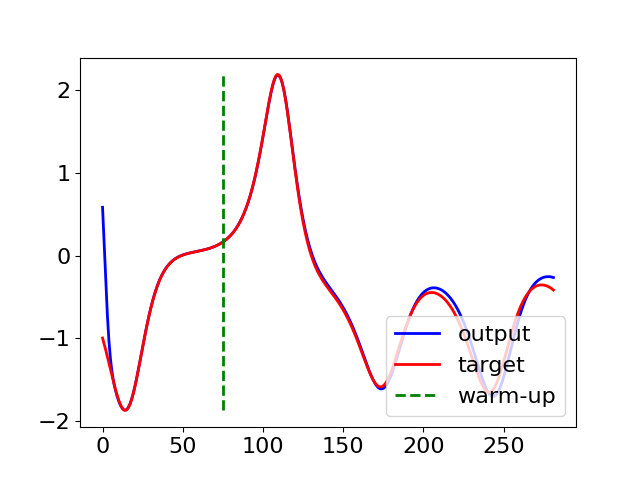
\includegraphics[width=\textwidth]{../Results/Lorenz-63/Figures/RNN-lstm-RDIM_3-N_used_50000-NUM-LAY_1-SIZE-LAY_100-ACT_tanh-ISH_statefull-SL_8-PL_4-LR_0.0001-DKP_1.0-ZKP_1.0-HSPL_300-IPL_200-NL_1-WID_0/prediction_augmend_TEST_33278.png}
			\caption{Prediction of first dimension}
		\end{subfigure}
%		\begin{subfigure}[b]{0.45\textwidth}
%			\includegraphics[width=\textwidth]{../\SixtyThreePath/prediction_TEST_\SixtyThreePathIndexOne_error.png}
%			\caption{Error of first dimension}
%		\end{subfigure}
		\begin{subfigure}[b]{0.45\textwidth}
			\includegraphics[width=\textwidth]{../\SixtyThreePath/prediction_TEST_\SixtyThreePathIndexOne.png}
			\caption{Predictions of all dimensions}
		\end{subfigure}
%		\begin{subfigure}[b]{0.5\textwidth}
		\begin{subfigure}[b]{\textwidth}
			\includegraphics[width=\textwidth]{../\SixtyThreePath/prediction_TEST_\SixtyThreePathIndexOne_contour.png}
			\caption{Contour plot}
		\end{subfigure}
		\caption{Test results for random initial condition \SixtyThreePathIndexOne}
		\label{63:predictions1}
	\end{figure}
	
	\begin{figure}[h]
		\centering
		\begin{subfigure}[b]{0.45\textwidth}
			\includegraphics[width=\textwidth]{../\SixtyThreePath/prediction_augmend_TEST_\SixtyThreePathIndexTwo.png}
			\caption{Prediction of first dimension}
		\end{subfigure}
%		\begin{subfigure}[b]{0.45\textwidth}
%			\includegraphics[width=\textwidth]{../\SixtyThreePath/prediction_TEST_\SixtyThreePathIndexTwo_error.png}
%			\caption{Error of first dimension}
%		\end{subfigure}
		\begin{subfigure}[b]{0.45\textwidth}
			\includegraphics[width=\textwidth]{../\SixtyThreePath/prediction_TEST_\SixtyThreePathIndexTwo.png}
			\caption{Predictions of all dimensions}
		\end{subfigure}
%		\begin{subfigure}[b]{0.45\textwidth}
		\begin{subfigure}[b]{\textwidth}
			\includegraphics[width=\textwidth]{../\SixtyThreePath/prediction_TEST_\SixtyThreePathIndexTwo_contour.png}
			\caption{Contour plot}
		\end{subfigure}
		\caption{Test results for random initial condition \SixtyThreePathIndexTwo}
		\label{63:predictions2}
	\end{figure}

	\FloatBarrier
\subsection{Lorenz-96}
	\newcommand{\NinetySixPath}{Results/Lorenz-96/Figures/RNN-lstm-RDIM_10-N_used_100000-NUM-LAY_3-SIZE-LAY_100-ACT_tanh-ISH_statefull-SL_8-PL_2-LR_0.0001-DKP_1.0-ZKP_1.0-HSPL_300-IPL_200-NL_1-WID_0}
	\newcommand{\NinetySixPathIndexOne}{25172}
	\newcommand{\NinetySixPathIndexTwo}{50168}
	
	\begin{figure}[h]
		\centering
		\begin{subfigure}[b]{0.45\textwidth}
			\includegraphics[width=\textwidth]{../\NinetySixPath/Loss_total_log.png}
			\caption{Training and validation loss}
			\label{96:loss}
		\end{subfigure}
		\begin{subfigure}[b]{0.45\textwidth}
			\includegraphics[width=\textwidth]{../\NinetySixPath/spectrum_comparison_TEST.png}
			\caption{Power spectrum for test predictions}
			\label{96:spectrum}
		\end{subfigure}
		\caption{Loss and power spectrum}
	\end{figure}

	Again \cref{96:loss} proves that the model learns and again no overfitting can be detected. However learning the Lorenz-96 proves to be significantly more difficult. This is to be expected, as this dataset is 10-dimensional, among other things. We therefore searched a lot for goot hyperparameters and also improved the learning rate scheduler, but the training always converged at a validation error of about 0.0011. The model's limited ability to predict the system is substantiated by the quality o the predictions of the test data. One can clearly see that only the first steps are correct but than prediction is off and evolves different. However, the Paper of Vlachas et alium, suggested that the LSTM should be able to fit to the Lorenz-96 system. This could be because we did not find the perfect hyperparameter. Futhermore, they used the stateless LSTM model while we used the statefull LSTM model. They also tried other models like the MSM or the combination MSM-LSTM. These models could eventually lead to better results. For the power spectrum we again use a smoothing factor $\sigma=50$ and a cutoff-frequency $f_{\text{cut}}=5000$. The spectra seems to fit well, but the differences are not clearly visible due to the peak at low frequencies.
	
	\begin{figure}[h]
		\centering
		\begin{subfigure}[b]{0.45\textwidth}
			\includegraphics[width=\textwidth]{../\NinetySixPath/prediction_augmend_TEST_\NinetySixPathIndexOne.png}
			\caption{Prediction of first dimension}
		\end{subfigure}
		\begin{subfigure}[b]{0.45\textwidth}
			\includegraphics[width=\textwidth]{../\NinetySixPath/prediction_TEST_\NinetySixPathIndexOne_error.png}
			\caption{Error of first dimension}
		\end{subfigure}
		%		\begin{subfigure}[b]{0.5\textwidth}
		\begin{subfigure}[b]{\textwidth}
			\includegraphics[width=\textwidth]{../\NinetySixPath/prediction_TEST_\NinetySixPathIndexOne_contour.png}
			\caption{Contour plot}
		\end{subfigure}
		\caption{Test results for random initial condition \NinetySixPathIndexOne}
		\label{96:predictions1}
	\end{figure}

	\begin{figure}[h]
		\centering
		\begin{subfigure}[b]{0.45\textwidth}
			\includegraphics[width=\textwidth]{../\NinetySixPath/prediction_augmend_TEST_\NinetySixPathIndexTwo.png}
			\caption{Prediction of first dimension}
		\end{subfigure}
		\begin{subfigure}[b]{0.45\textwidth}
			\includegraphics[width=\textwidth]{../\NinetySixPath/prediction_TEST_\NinetySixPathIndexTwo_error.png}
			\caption{Error of first dimension}
		\end{subfigure}
		\begin{subfigure}[b]{\textwidth}
			\includegraphics[width=\textwidth]{../\NinetySixPath/prediction_TEST_\NinetySixPathIndexTwo_contour.png}
			\caption{Contour plot}
		\end{subfigure}
		\caption{Test results for random initial condition \NinetySixPathIndexTwo}
		\label{96:predictions2}
	\end{figure}
	